\documentclass[tikz,border=8pt]{standalone}
\usepackage{amsmath}
\usetikzlibrary{arrows.meta,positioning,fit}

\begin{document}
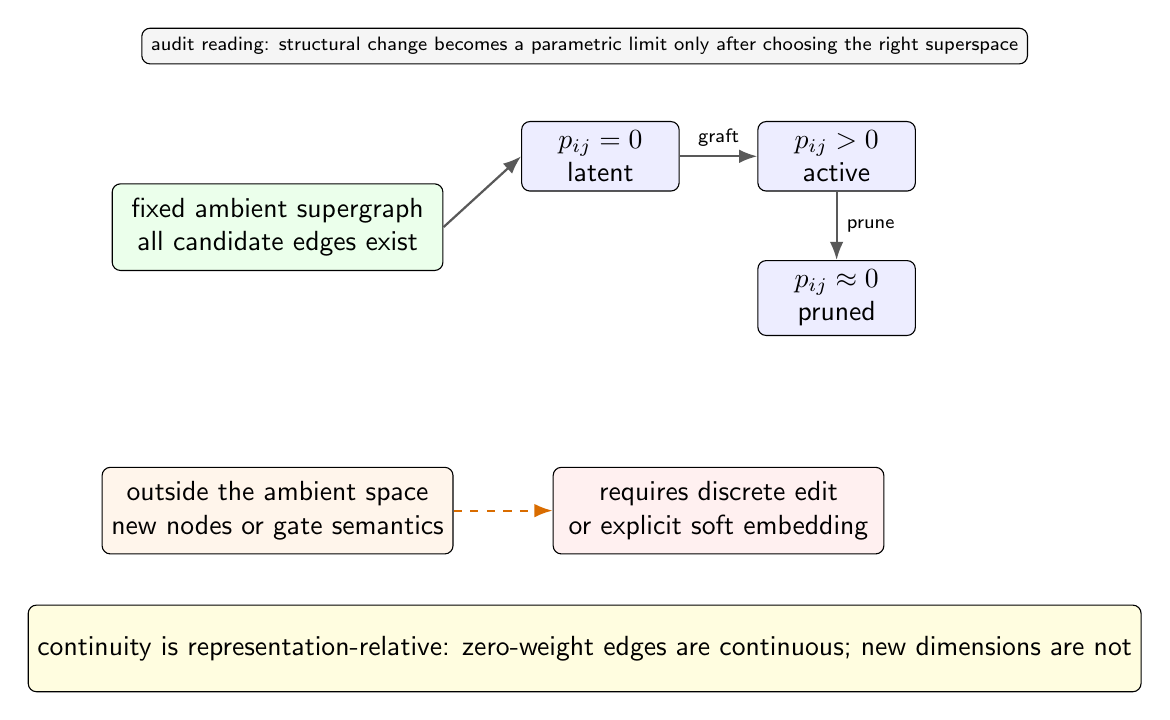
\begin{tikzpicture}[
  font=\sffamily,
  box/.style={draw, rounded corners=3pt, align=center, minimum width=42mm, minimum height=11mm, fill=white},
  small/.style={draw, rounded corners=3pt, align=center, minimum width=20mm, minimum height=8mm, fill=white},
  note/.style={align=center, font=\sffamily\scriptsize},
  arrow/.style={-Latex, thick, draw=black!65},
  warn/.style={-Latex, thick, dashed, draw=orange!85!black}
]

\node[box, fill=green!8] (ambient) at (0,1.8)
  {fixed ambient supergraph\\all candidate edges exist};
\node[small, fill=blue!7] (zero) at (4.1,2.7) {$p_{ij}=0$\\latent};
\node[small, fill=blue!7] (active) at (7.1,2.7) {$p_{ij}>0$\\active};
\node[small, fill=blue!7] (dead) at (7.1,0.9) {$p_{ij}\approx0$\\pruned};

\draw[arrow] (ambient.east) -- (zero.west);
\draw[arrow] (zero) -- node[above, note] {graft} (active);
\draw[arrow] (active) -- node[right, note] {prune} (dead);

\node[box, fill=orange!8] (outside) at (0,-1.8)
  {outside the ambient space\\new nodes or gate semantics};
\node[box, fill=red!6] (lift) at (5.6,-1.8)
  {requires discrete edit\\or explicit soft embedding};
\draw[warn] (outside) -- (lift);

\node[box, fill=yellow!12, minimum width=78mm] at (3.9,-3.55)
  {continuity is representation-relative: zero-weight edges are continuous; new dimensions are not};

\node[note, fill=gray!8, draw, rounded corners=3pt, minimum width=86mm] at (3.9,4.1)
  {audit reading: structural change becomes a parametric limit only after choosing the right superspace};

\end{tikzpicture}
\end{document}
